%! TEX root = main.tex

\graphicspath{{00_Images/12_chapter/}}

\chapter{Power Amplifiers Output Stages}
\label{ch:poweramp}

\section{Introduction to Power Amplification}
\label{sc:121}

The power amplifier is the last block of the audio chain, the stage that finally drives the loudspeaker after the signal has been preamplified, filtered, equalized, and processed.
Its task is fundamentally different from that of the stages that precede it.
Where a preamplifier provides voltage gain, the power stage provides almost none, with a voltage gain close to unity, and is instead responsible for current amplification: it must deliver the large currents required by a very low impedance load, the loudspeaker being typically a \SI{4}{\ohm} or \SI{8}{\ohm} device.
For this reason the power stage is configured as a voltage buffer, the solid-state counterpart of the valve output stage of chapter \ref{ch:valves}, with a voltage gain \(G_V \approx 1\) and a current gain \(G_I \gg 1\).

Delivering tens of volts and several amperes calls for dedicated power transistors, complementary bipolar pairs such as the MJ15003 and MJ15004, mounted on heat sinks to dissipate the considerable heat generated.
Every such device is constrained by its safe operating area, the region of the voltage-current plane within which it can operate without damage: the product of the collector-emitter voltage and the collector current must stay below the maximum power-dissipation limit, so the operating point can never cross the iso-power boundary of the device.

\begin{figure}[!htb]
    \centering
    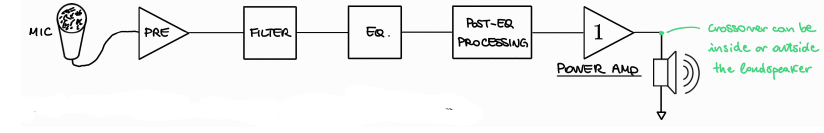
\includegraphics[width=0.75\textwidth]{Signal_Chain.png}
    \caption{Position of the power amplifier as the final block of the audio chain, driving the loudspeaker}
    \label{fig:signalChain}
\end{figure}

The amplifier classes, Class A, Class B, Class AB, and Class D, differ in how the output devices are biased and how each conducts over the signal cycle, a choice that trades linearity against efficiency.

\section{Class A Amplifier}
\label{sc:122}

The Class A stage is built on the emitter-follower architecture analyzed in section \ref{sc:74}, in which a single transistor, or a set acting as one, conducts current throughout the entire cycle of the waveform, for the full \(360^\circ\).
As an emitter follower its voltage gain is essentially unity,
\[
A_V = \frac{v_{out}}{v_{in}} = \frac{g_m R_L}{1 + g_m R_L} \approx 1 \quad \text{for } g_m R_L \gg 1
\]
the same near-unity transfer met in the Tube Screamer buffer of chapter \ref{ch:tubescreamer}, while its current gain is large, \(A_I = i_E/i_B = \beta + 1\), confirming that the stage amplifies current rather than voltage.

\begin{figure}[!htb]
    \centering
    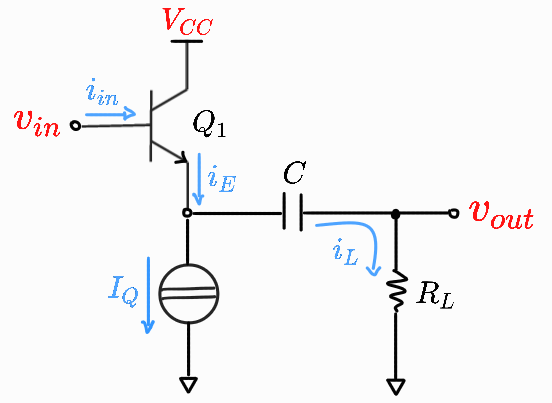
\includegraphics[width=0.50\textwidth]{Class_A_Stage.png}
    \caption{Class A output stage in emitter-follower configuration, with the load AC-coupled through the capacitor}
    \label{fig:classA}
\end{figure}

\paragraph{Supply requirements} A numerical example fixes the orders of magnitude.
To deliver \(P_L = \SI{100}{\watt}\) into \(R_L = \SI{8}{\ohm}\), the load voltage must reach \(v_{RMS} = \sqrt{P_L R_L} = \SI{28.3}{\volt}\), a peak \(\hat{V}_L = \sqrt{2} v_{RMS} \approx \SI{40}{\volt}\), so the supply must satisfy \(V_{CC} \geq 2\hat{V}_L = \SI{80}{\volt}\).
The corresponding peak load current is \(\hat{i}_L = \hat{V}_L/R_L = \SI{5}{\ampere}\), drawn from an input base current of only \(\hat{i}_{in} = \hat{i}_L/(\beta + 1) \approx \SI{50}{\milli\ampere}\), which again illustrates the large current gain of the stage.

\paragraph{Efficiency} The efficiency of any output stage is the ratio of the average power delivered to the load to the average power drawn from the supply:
\[
\eta = \frac{P_L}{P_S} \in [0, 1]
\]
For a sinusoidal output at maximum swing the peak load voltage reaches \(\hat{V}_L = V_{CC}/2\), so the load power is
\[
P_L = \frac{\hat{V}_L^2}{2 R_L} = \frac{V_{CC}^2}{8 R_L}
\]
The supply, on the other hand, must sustain a constant quiescent current at all times, because in Class A the device never switches off.
The sinusoidal load current averages to zero, so the average supply current equals the quiescent current, which must be at least \(I_Q = V_{CC}/(2 R_L)\) to feed the negative half-cycle, giving
\[
P_S = V_{CC} \overline{I_S} = V_{CC} \cdot \frac{V_{CC}}{2 R_L} = \frac{V_{CC}^2}{2 R_L}
\]
The maximum efficiency is therefore
\[
\eta_{max} = \frac{V_{CC}^2 / (8 R_L)}{V_{CC}^2 / (2 R_L)} = \frac{1}{4} = 25\%
\]
The Class A stage thus delivers an extremely linear, low-distortion signal, since the single device handles the whole waveform without switching, but it wastes at least three quarters of the supply power as heat, dissipated continuously even when no signal is present.

\section{Class B Amplifier}
\label{sc:123}

The waste of Class A comes from the permanent quiescent current, and the Class B stage removes it by splitting the work between two complementary transistors in a push-pull configuration.

\begin{figure}[!htb]
    \centering
    \subfloat[Push-pull output with complementary NPN and PNP devices]{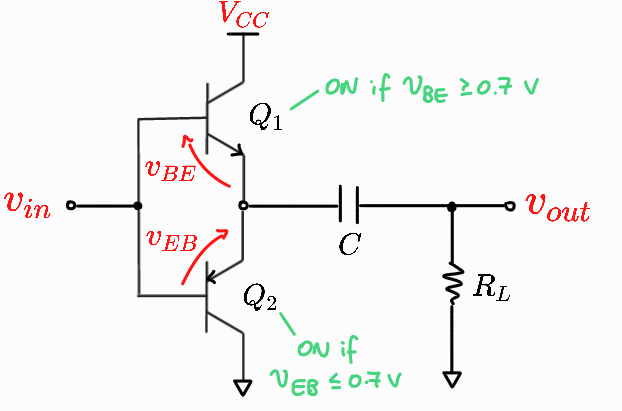
\includegraphics[height=0.18\textheight]{Class_B.png}}
    \hfill
    \subfloat[Transfer characteristic showing the crossover dead zone around the origin]{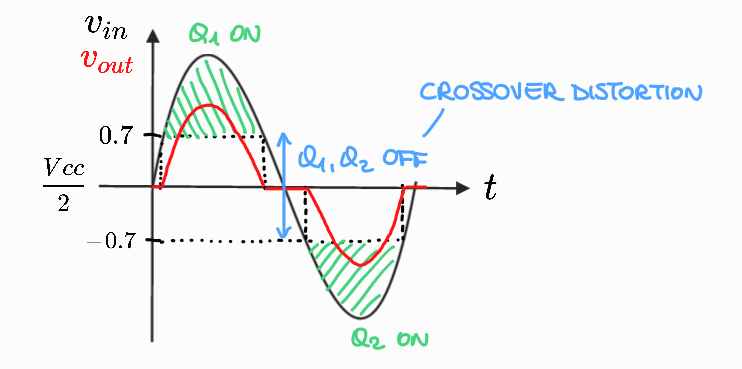
\includegraphics[height=0.18\textheight]{class_B_graph.png}}
    \caption{Class B push-pull stage and the crossover distortion produced by the conduction dead zone}
    \label{fig:classB}
\end{figure}

In the push-pull arrangement of figure \ref{fig:classB} an NPN transistor handles the positive half-cycle and a complementary PNP transistor handles the negative one, so each device conducts for only \(180^\circ\) and neither carries any current at idle.
With no quiescent current the supply power follows the signal, and the efficiency rises sharply.
The supply current is now a rectified sine of peak \(\hat{i}_L = V_{CC}/(2 R_L)\), whose average over the cycle is \(\overline{I_S} = V_{CC}/(2\pi R_L)\), so the supply power is
\[
P_S = V_{CC} \overline{I_S} = \frac{V_{CC}^2}{2\pi R_L}
\]
and the maximum efficiency becomes
\[
\eta_{max} = \frac{V_{CC}^2 / (8 R_L)}{V_{CC}^2 / (2\pi R_L)} = \frac{\pi}{4} \approx 79\%
\]
more than three times that of Class A.

\paragraph{Crossover distortion} The push-pull stage pays for its efficiency with a characteristic nonlinearity.
A bipolar transistor begins to conduct only once its base-emitter voltage reaches about \SI{0.7}{\volt}, so the NPN device turns on for \(v_{in} \geq \SI{0.7}{\volt}\) and the PNP device for \(v_{in} \leq \SI{-0.7}{\volt}\).
Between these two thresholds, across a dead zone of \SI{1.4}{\volt} centered on the origin, neither transistor conducts and the output stays flat.
The result is a sharp step in the transfer characteristic at every zero crossing of the waveform, the crossover distortion of figure \ref{fig:classB}, which is most audible on low-level signals where the dead zone occupies a large fraction of the swing.

\section{Class AB Amplifier}
\label{sc:124}

The industrial solution to crossover distortion is the Class AB stage, a push-pull output in which both devices are kept slightly conducting at all times.
A small DC bias, of the order of the \SI{0.7}{\volt} threshold, is applied between the two bases by a string of diodes or by a \(V_{BE}\) multiplier, so that each transistor is already on the verge of conduction when the signal crosses zero.
The dead zone disappears, and one device pushes current into the load while the other pulls it, with a smooth handover at the crossing point.

\begin{figure}[!htb]
    \centering
    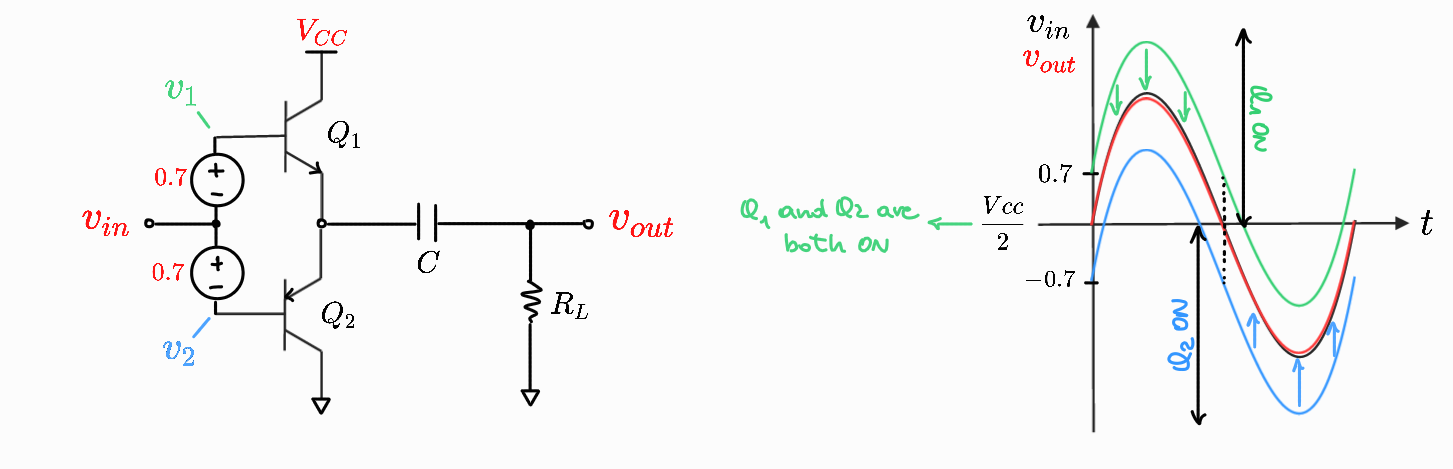
\includegraphics[width=0.80\textwidth]{Class_AB_Stage.png}
    \caption{Class AB output stage: a small bias between the bases keeps both devices weakly on, removing the crossover step while retaining the push-pull efficiency}
    \label{fig:classAB}
\end{figure}

Class AB therefore combines the high efficiency of Class B, close to the same \(\pi/4\) bound, with the low distortion of Class A, and it is the topology of the great majority of analog audio power amplifiers.
Because the small idle current makes the bias sensitive to temperature, the stage must include a bias-compensating network to prevent thermal runaway, in which a rising junction temperature increases the current and further raises the temperature.

\paragraph{Case study: the Luxman 900u} A high-end realization of these principles is the Luxman 900u integrated amplifier, which operates in Class AB with a dual-mono, symmetric layout.
Its output stage uses several complementary push-pull pairs connected in parallel, so that the very large load current, of the order of \SI{16}{\ampere} at full output, is shared among the paralleled devices rather than forced through a single transistor, keeping each one within its safe operating area.
The bias is set so that the amplifier runs in pure Class A at low levels and transitions to Class AB as the output grows, while current-sensing resistors and protection circuits guard the output devices against short circuits and fault conditions.

\paragraph{A note on Class D} Beyond the linear classes, the Class D amplifier achieves efficiencies approaching \(100\%\) by operating its output devices as switches rather than as linear current sources.
The signal is encoded as a pulse-width-modulated waveform that toggles the output between the supply rail and ground, and a passive LC low-pass filter then recovers the audio by extracting the average value.
Because the switching devices are either fully on or fully off, they dissipate almost no power, which makes Class D the dominant choice in modern powered loudspeakers and portable systems where efficiency and weight are paramount.
